% !TEX root =  ../report.tex

\section{Implementation}
The OP2 library is hosted open source on GitHub\cite{OP2rep}. Instructions for obtaining the implementation completed for this report, and getting started with OP2 can be found in Appendix \ref{app:getStart}.
\par
The feature branch for this project, \verb|feature/jit| was branched from \\\verb|feature/lazy-execution| on 13th November 2019. The \verb|laxy-execution| branch's last commit was in April 2018, and lagged behind the \verb|master| branch somewhat. It was rebased onto \verb|master| before any other changes were made.
\par
The \verb|lazy-execution| branch contained the beginnings of a system to execute parallel loops when values are required rather than when called. This is done through an internal library function:
\codeline{void op_enqueue_kernel(op_kernel_descriptor *desc)}{op2/c/src/core/op\_lazy.cpp [71-89]}
Which currently simply executes the function straight away. This process for calling parallel loops is used similarly throughout work done to enable Just In Time Compilation for CUDA, so that future efforts towards lazy execution can continue in the future on top of the JIT implementation.

\subsection{Code Generation}
The Python code generation script which forms the main body of the implementation can be found in: \verb|translator/c/python/jit/op2_gen_cuda_jit.py|
\\
The main function is:
\pyline{def op2_gen_cuda_jit(master, date, consts, kernels)}{translator/c/python/jit/op2\_gen\_cuda\_jit.py [102]}
Which is called from \verb|op2.py| in the parent directory - the same as the other code generation scripts. It's parameters are:\\
\begin{tabular}{>{\bfseries}l l}
  master: & The name of the Application's master file \\
  date: & The exact time of code generation \\
  consts: & list of constants, with their type, dimension and name \\
  kernels: & \parbox[t]{.8\textwidth}{list of kernel descriptors, where each kernel is a map containing many fields describing the kernel, which may alter the way the code for that loop is generated.}
\end{tabular}
\\
\par
The code generator first performs a quick check across all kernels to see if any use the Struct of Arrays feature \cite[p9]{manual}, or if all are using the default data layout. Then iterates over each kernel, and generates both the Ahead Of Time (AOT) kernel file, and the Just In Time (JIT) kernel file simultaneously. A folder \verb|cuda| is created if it doesn't exist, and two files generated in it for each kernel:
\begin{itemize}
\item{\verb|AOT: cuda/[name]_kernel.cu|}
\item{\verb|JIT: cuda/[name]_kernel_rec.cu|}
\end{itemize}

\begin{figure}[h!]
\centering
\begin{minipage}{.55\textwidth}
Some sections of both files are the same. The examples in Figure \ref{fig:jit_include} show the progression of each file for an example kernel.
\\\\ The first thing generated is simply the include directives required for the JIT compiled kernel. These are needed since they will be compiled seperately:
\begin{footnotesize}
\lstset{xleftmargin=.25in}
\begin{lstlisting}
#include "op_lib_cpp.h"
#include "op_cuda_rt_support.h"
#include "op_cuda_reduction.h"
//global_constants
#include "jit_const.h"
\end{lstlisting}
\end{footnotesize}
The \verb|jit_const.h| file is also included, which will be generated at runtime (before the compiler is invoked) to \verb|#define| constants for the preprocessor.
\end{minipage}
\hfill
\begin{minipage}{.4\textwidth}
  \centering
  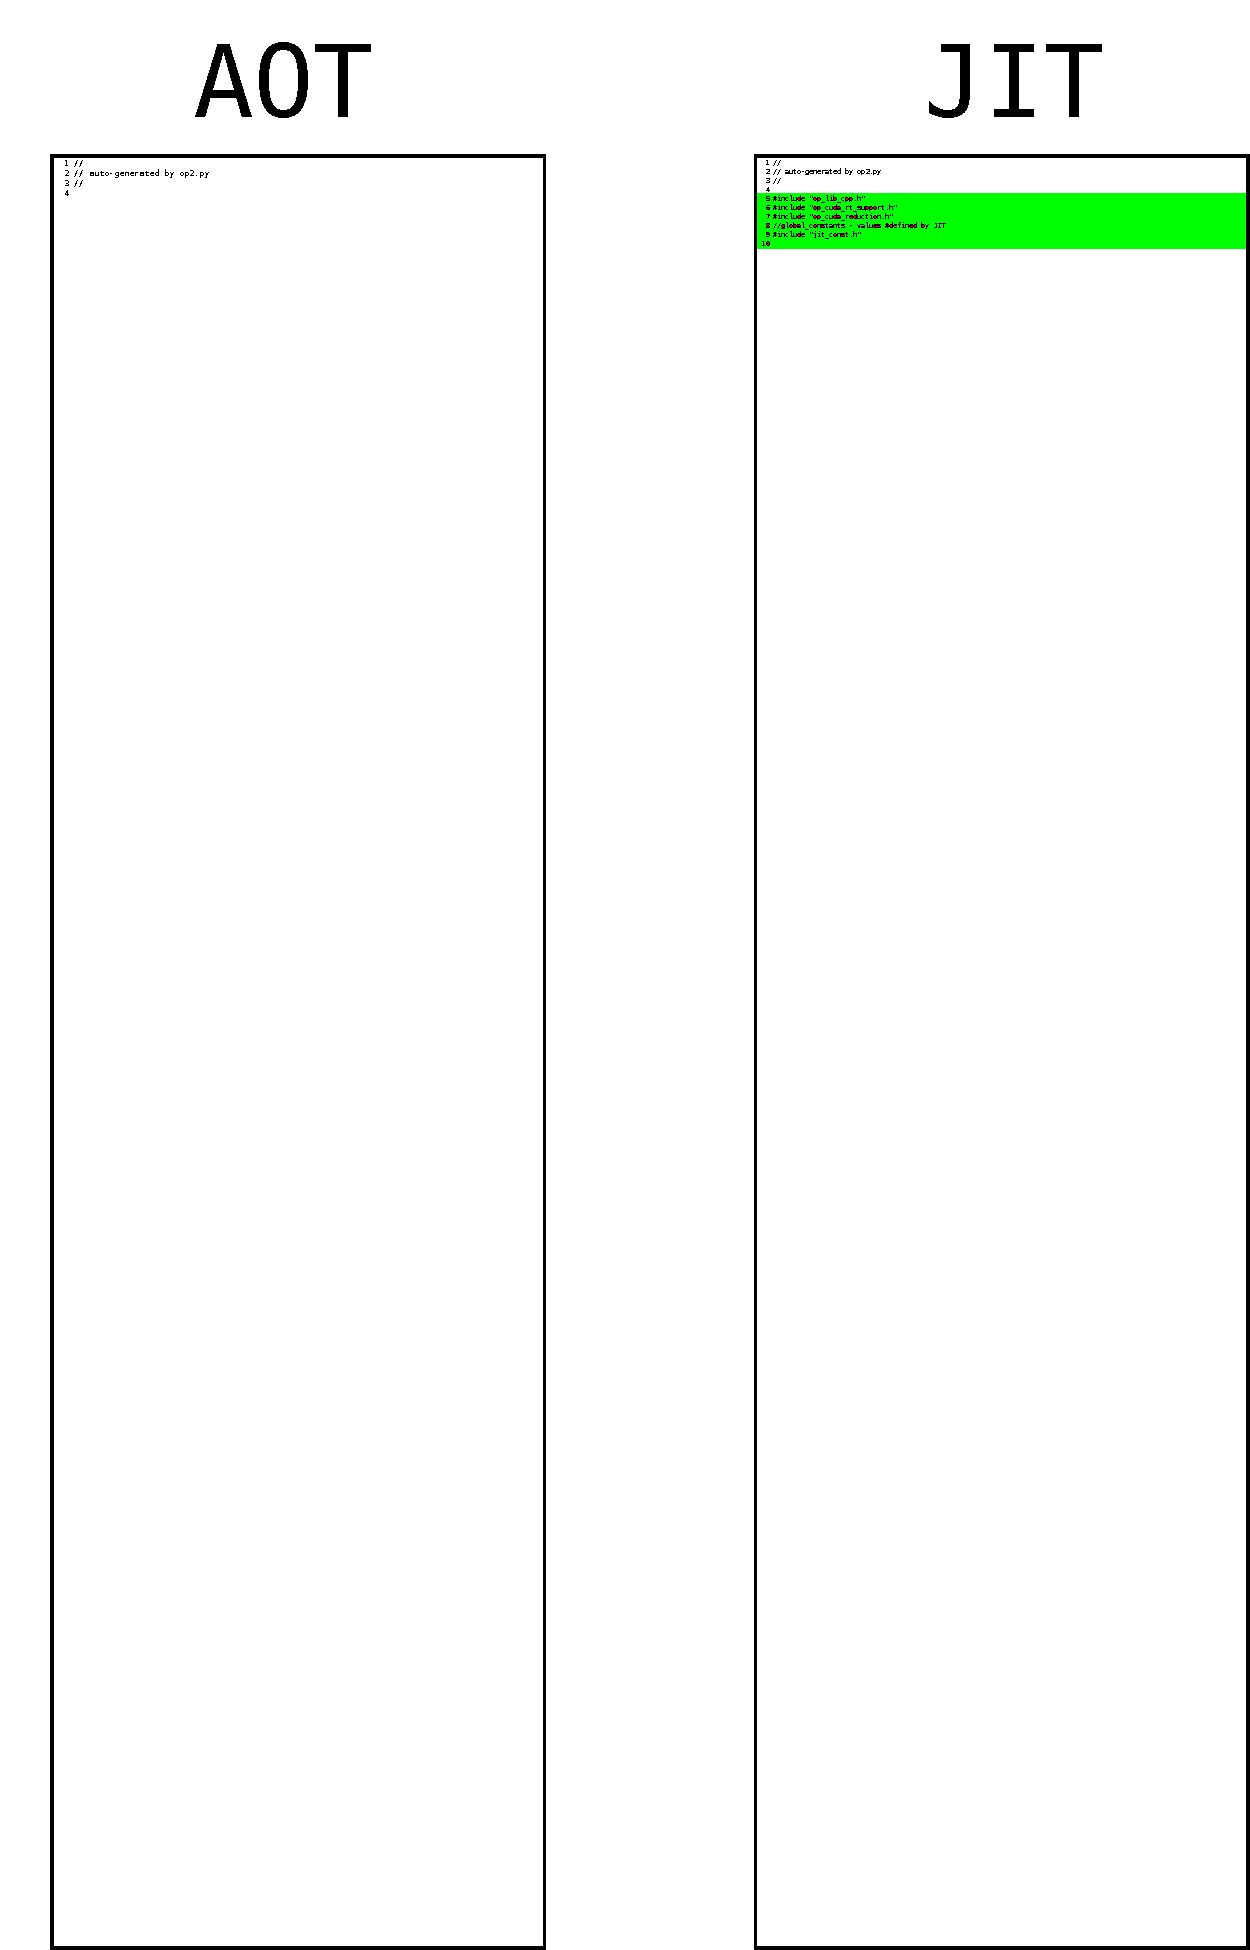
\includegraphics[width=\textwidth]{jit_include}
  \caption{JIT includes}
  \label{fig:jit_include}
\end{minipage}%
\end{figure}
